\chapter{Preliminaries}

% Firstly, I should introduce the notations, definitions and properties which are necessary to understand this report, including
% Database: relations, schemes, attributes, size of relations
% Definition of joins (conjunctive query)


% notations
In this chapter, the notations, definitions and properties which are necessary to understand the report are introduced. 

\paragraph{Databases.} A relation schema is a finite set of attributes and for an attribute $A$, we use $dom(A)$ to denote its domain. A tuple $t$ over a relation schema $S$ is a mapping from the attributes in $S$ to data values. A relation over a relation schema $S$ is a finite set of tuples over $S$. Let $\D$ be a relational database of $n$ relations $R_1, ..., R_n$, where each $R_i$ has a relation schema $S(R_i)$. The size of a relation $R$, denoted by $|R|$, is the number of tuples in the relation and the size of the database $|\D|$ is the sum of the sizes of the relations. 

% joinable

% conjunctive query
\paragraph{Join Queries.}
Let $Q$ be a conjunctive query. The query $Q$ can be written in the relational algebra form $Q = \pi_{\calP}(\sigma_{\psi}(R_1 \times ... \times R_n))$, where each $R_i$ corresponds to a relation occurring in the database and the selection condition $\psi$ is a conjunction of equalities of the form $A_1 = A_2$ with attributes $A_1$ and $A_2$, and the projection list $\calP$ is a subset of $\bigcup_i S(R_i)$. The equivalence class $\calA$ of an attribute $A$ is the set consisting of $A$ and of all attributes equivalent to $A$ in $\psi$. If $\calP = \bigcup_i S(R_i)$ we can drop the projection operator and $Q = \sigma_{\psi}(R_1 \times ... \times R_n)$ is called an equi-join query. 

The result of the query $Q$ over database $\D$ is denoted by $Q(\D)$ and it is obtained as follows: for each possible assignment $\alpha$ of the Cartesian product of the relations in the database, if $\alpha$ satisfies all the equalities in $\psi$, the tuple $\alpha$ is in $Q(\D)$.
% For convenience, we use a single attribute to represent all attributes in the same equivalence class to avoid duplication. For example, for the query $Q$ with a selection condition containing $R_1.A = R_2.A$, since they have the same values, we use $A$ to represent all of them. 


\paragraph{Listing and Factorised Representations.}
Two methods of the representation of data in databases are discussed in this report: listing representations and factorised representations. The listing representations is the method applied by most of commercial Relational Database Management Systems (RDBMSs) which stores data tuple by tuple. However, this method has been shown to be sub-optimal in that single values or even blocks of values are stored unnecessarily repeatedly. For example, (TODO). 

To get rid of redundancy, factorised representations are proposed which factor the common values out and store them only once. 
% To get rid of this redundancy, factorised representations are proposed. 
Formally, factorised representations consist of operators in relational algebra including union, Cartesian product and so-called singletons which are unary relations with only one tuple: $\tuple{A:a}$ where $A$ is the attribute of the relation and $a$ is its value. A listing representation can be encoded into a factorised representation as the union of products of singletons. To remove the redundancy in it, we exploit the distributivity and commutativity of product over union to factor out common sub-expressions and nest products and unions in order to avoid expressing those sub-expressions repeatedly. Then, we can further compress the representation by using references to define repeated sub-expression that cannot be factored out algebraically only once. An important property of factorised representations is that tuples in a factorised representation can be enumerated with constant delay, which means they can enumerate in the same time complexity as the listing representations, despite that fact that factorised representations can be exponentially smaller. 

(TODO, an example showing the factorised representation is succinct)The figure shows an example that a factorised representation can be much more succinct than a listing representation and it can be further compressed by applying referencing. 


\section{Hypergraph}
% strategy is important
We can gain information by analysing the properties of a given query and the relations which are useful for us to develop join strategies before performing the join. We use hypergraphs and hypertree decomposition to represent the structure information of queries. 


A hypergraph $\calH$ is a pair $(\calV, \calE)$  where $\calV$ is a set of nodes and $\calE$ is a set of non-empty sets of nodes named hyperedges. A hypergraph $\calH$ of a query $Q$ consists of one node for each attribute $A$ in $Q$ and one edge for the schema $S(R)$ of each relation $R$ in $Q$. The attributes in the same relation have pairwise connections between each other. We capture those connections by putting attributes in the same relation into the same hyperedge. 


\paragraph{Example \ref{example:triangle}}\label{example:triangle}
The triangle query: Given a database $\D$ with three relations $R(A,B)$, $S(B,C)$ and $T(C,A)$, and the triangle query is a equi-join
$$Q = \sigma_{\psi}(R(A,B)\times S(B,C) \times T(C,A))$$
where $\psi$ is $R.A = T.A \land R.B = S.B \land S.C = T.C$. For convenience, we use a single attribute to represent the attributes in the same equivalence class. In this example, we can use $A$ to represent $R.A$ and $T.A$, $B$ to represent $R.B$ and $S.B$, and $C$ to represent $S.C$ and $T.C$, so the underlying hypergraph of the triangle query $Q$ is $\calH = (\set{A,B,C}, \set{\set{A,B}, \set{B,C}, \set{C,A}})$ which is shown in the Figure \ref{fig:triangle}. 

% \begin{figure}[t]
% 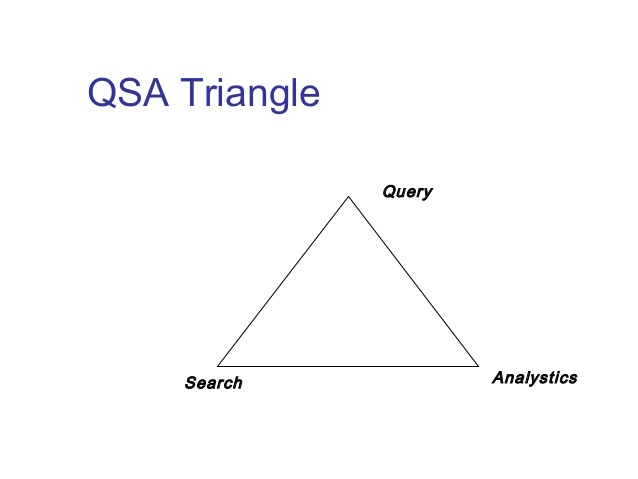
\includegraphics[scale=0.4]{chapters/images/triangle.jpg}
% \centering
% \caption{Triangle query for the Example \ref{example:triangle}}
% \label{fig:triangle}
% \end{figure}



\paragraph{Example \ref{example:path4}}\label{example:path4}
Another example is named path query: Given a database $\D$ with four relations $R(A,B)$, $S(B,C)$ and $T(C,D)$, and the path query is a equi-join with the selection condition $R.B=S.B \land S.C=T.C$. The hypergraph of the query is shown in the right of the Figure \ref{fig:triangle}. 


TODO: 
the triangle query and path query figures 
the reference number of examples

compares the path4 and triangle (cyclic)




\section{Hypertree Decomposition}
Formally, a tree decomposition $\calT$ of a hypergraph
$\calH = (\calV, \calE)$ of a Q is a pair $(T, \calX)$ such that $T$ is a tree and $\calX$ is a function mapping each node in $T$ to a subset of $\calV$ which is called bag. A decomposition $\calT$ satisfies two properties, which are 
\begin{itemize}
  \item Converge: $\forall e \in \calE$, there must be a node $t \in T$ such that $e \subseteq \calX(t)$. 
  \item Connectivity: $\forall v \in \calV, \set{t \mid t \in T, v \in \calX(t)}$ forms a connected subtree. 
\end{itemize}

A tree decomposition is called reduced if there does not exist a bag which is the subset of another bag. The width of a tree decomposition $(T, \calX)$ is defined as the size of the largest bag minus one: $\max_{t \in T}{(|\calX(t)| - 1)}$ and the treewidth $tw(\calH)$ of the hypergraph $\calH$ is the minimum width over all possible tree decompositions. 


A generalised hypertree decomposition of a hypergraph $\calH$ is a triple $(T, \calX, \set{\gamma}_{t \in T})$, where $(T, \calX)$ is a tree decomposition of $\calH$ and for each node $t \in T$, $\gamma_t$ denotes a subset of $\calE$ such that $\calX(t) \subseteq \bigcup_{e \in \gamma_t}e$. That is, for each bag in $\calX$, all nodes in the bag are covered by the hyperedges in the corresponding $\gamma_t$. A hypertree decomposition is a special generalised hypertree decomposition with the condition: $\forall t \in T, \forall e \in \gamma_t, e \cap \calX(T_t) \subseteq \calX(t)$, where $T_t$ is the subtree of $T$ rooted at $t$ and $\calX(T_t) = \bigcup_{t \in T_t}\calX(t)$. 

The width of a (generalised) hypertree decomposition $(T, \calX, \set{\gamma}_{t \in T})$ is defined as the size of the largest $\gamma_t$: $\max_{t \in T}(|\gamma_t|)$. The width of a tree decomposition $\calT = (T, \calX)$ is defined as the minimal width of all possible hypergraph decompositions which are extensions of $\calT$ by $\set{\gamma}_{t \in T}$. Similarly, the hypertree width $htw(\calH)$ of a hypergraph $\calH$ is the minimal width over all possible hypertree decompositions. 


In this report, it is not unnecessary to distinguish between the generalised hypertree decomposition and the hypertree decomposition. [TODO:] proved the width of a generalised hypertree decomposition is always ... . For simplify, I use only hypertree decomposition in this report. 

The tree decomposition method simplifies a hypergraph by putting the attributes generating cycles in bags so that there is not a cycle in the generated tree. The hypergraph $\calH$ is acyclic when it has a tree decomposition in which each bag is subsumed in an hyperedge of $\calH$ []. The width of a query denotes its degree of cyclicity, which intuitively measures how far it is from an acyclic query. The width of an acyclic query is always $1$.  

% Yannakakis

TODO
Examples 
- triangle
- path


\section{Variable Orders}
% assume factorised representations are introduced in the introduction chapter and the key of the factorised representations are sharing based on the conditional independencies. (similar to the sumprod)
% suggest: factorisation => branching => succinct representation






% variable order something
% how to get factorised representation from variable orders
% how to apply those representations






% The succinctness of factorised representations comes from the branching of attributes and the referencing of common sub-expressions. The key condition of allowing more branching and referencing is the conditional independencies of the attributes. Two attributes are conditional independencies iff TODO. 

% how to get the best 
% the succinct comes from branching and sharing
% => independent is where branching comes from
% => independent is analysed in [OZ15] and defined
% => so to get the independent information is important
% => so we need structure information 


% TODO: the example: a listing representation and its corresponding factorised representation



Similar to hypertree decompositions, variable orders (d-trees) of a query is a representation capturing the structure information of the query. There exists algorithms for bidirectional translation between a variable order and a hypertree decomposition, which proves they have the same representation ability. Variable orders are convenient for the algorithms of factorised representations since they specify partial orders of attributes and encode structural information that defines the conditional independencies of attributes which is the key condition of factoring and referencing in factorised representations.  

Formally, a variable order $\Delta$ for a query $Q$ is a pair $(F, key)$, where $F$ is a rooted forest with one node per attribute in $Q$ and $key$ is a function mapping each attribute $A$ to a subset of its ancestor attributes in $F$. A variable order $\Delta$ for $Q$ has two properties:

\begin{itemize}
  \item For each relation in $Q$, its attributes lie along the same root-to-leaf path in $F$ and for any such attributes $A$ and $B$, $A \in key(B)$ if $A$ is an ancestor of $B$. 
  \item For every child $B$ of $A$, $key(B) \subseteq key(A) \cup \set{A}$. 
\end{itemize}

TODO:
Examples
% - triangle
% - path

Variable orders can be used as the structure of factorised representations. Without considering the referencing, the factorised representation following a variable order $\Delta = (F, key)$ is the ground expression of $F$ with respect to the singletons in the database. 

Intuitively, the succinctness of factorised representations comes from the branching of attributes and the referencing of common sub-expressions. A branching in the variable order represents conditional independence between the attributes of the different subtrees and in the factorised representation, this independence is denoted as a product of unions instead of materialising all possible combinations of the independent attributes. Furthermore, the conditional independence exists also in the attributes in the same root-to-leaf path which is captured by $key$ sets. Attributes with the same $key$ sets are conditional independent so the expressions of them are always identical. In factorised representation, this independence is denoted as the referencing rather than storing them repeatedly. 





% The key condition of allowing more branching and referencing is the conditional independencies of the attributes. Two attributes are conditional independencies iff TODO. 

% The structure of factorised representations, which is named variable order, is defined as a partial order on the schema. A factorised representation without referencing is the ground expression of its variable order with respect to the singletons in the database. Different variable orders lead to factorised representations with different sizes, so it is important to find the variable order leading to the most succinct factorised representation. 






% The algorithm for translating a variable order $\Delta$ to a hypertree decomposition $\calT$ is that:
% Do I need to write down the algorithm for the bidirection translation?

